\documentclass[../main.tex]{subfiles}
\hbadness=1000000
\vbadness=1000000
\begin{document}
% In this chapter, we cover the study we have conducted on information transmission in cortical networks.
% This work was materialized in the scientific publication bearing the same title as this chapter: \textit{Information transmission in delayed neuronal circuits in the presence of a relay population} \citep{sanchez-claros_information_2021}.
% The main characteristic of these types of circuit is that they exhibit zero-time synchronization despite being distant areas from each other; in other words, there are non-negligible delays primarily due to the length of the axons connecting these areas.
% Therefore, a fundamental piece of this work in this chapter is synchronization, and the fundamental question that motivated us is under what conditions a network exhibiting zero-time synchronization can efficiently transmit information.
\section{Introduction}
This chapter constitutes the third part of this thesis, which focuses on the design of a multicompartmental model of the hippocampus involving the CA3 and CA1 regions.
Our primary objective revolved around the theoretical exploration of the interplay between theta and gamma rhythms.
Theta and gamma rythms have been associated to memory formation in the hippocampus.
Examining the interaction between these distinct rhythms within CA3 and CA1 subregions offers valuable insights into how the brain organizes and processes information.
Through our model, we delve into this dynamic relationship, seeking to comprehend the fundamental mechanisms governing these rhythms and their potential impact on hippocampal function.
\subsection{The hippocampus}
The hippocampus is one of the most studied brain areas in mammals for two principal factors: it plays a fundamental role in learning, memory and spatial navigation, and it has a distinctive and identifiable layered structure that facilitates the conduct of electrophysiological recordings \citep{squire_medial_1991,witter_spatial_2006,buzsaki_memory_2013,eichenbaum_role_2017}.

% The hippocampal formation encompasses the hippocampus itself but also the surrounding regions that offer functional support to this structure.
% The hippocampus, an ancient structure in evolutionary terms known as \textit{archicortex}, is characterized by its three-layered composition.
The hippocampal formation is a compound structure in the medial temporal lobe of the brain that encompasses the \textbf{hippocampus}, the \textbf{dentate gyrus} (DG) and the \textbf{entorhinal cortex} (EC).
The hippocampus is made up of three distinct subfields: the Cornu Amonis 1, 2, and 3 (CA1, CA2, CA3).
In the CA regions, principal cells, known as \textbf{pyramidal cells}, are primarily located within a thin layer known as the \textit{stratum pyramidale} (SP), where their soma reside \citep{amaral2007hippocampal,buzsaki_memory_2013,lefebvre_development_2015}.
The basal dendrites and axons of these pyramidal cells are positioned dorsally in a layer called the \textit{stratum oriens} (SO), while their apical dendrites extend ventrally into the \textit{stratum radiatum} (SR) and further into the \textit{stratum lacunosum-moleculare} (SLM).
Beyond the pyramidal cells, the hippocampus boasts a diverese array of GABA-ergic interneurons which play essential roles in neural circuits \citep{petilla2008petilla,booker_morphological_2018, klausberger_gabaergic_2009}.

As shown in Figure \ref{fig:hippocampus_structure}, below the CA1 field, we find the dentate gyrus, a structured region characterized by three layer which is predominantly composed of glutamatergic granule cells placed within the \textit{stratum granulare} (SG).
The outer layer, referred as the \textit{stratum moleculare} primarily contains fibers projecting from the Entorhinal Cortex (EC).
In contrast, the inner layer, the \textit{stratum multiforme} (SM) or hilus, comprisses excitatory mossy cells \citep{amaral2007hippocampal,buzsaki_memory_2013,lefebvre_development_2015}.

The EC, situated laterally adjacent to the hippocampus, is a neocortical structure characterized by six distinct layers.
Functionally, it serves as a primary hub linking the broader neocortical regions with the archicortical networks of the hippocampus. 
The supperficial layers of the EC, layer II and III (ECII and ECIII) are responsible for projecting highly processed multisensory information into the hippocampus,
whereas layer V (ECV) receive projections from the hippocampus and subsequently relay this information to other cortical and subcortical regions \citep{amaral2007hippocampal,buzsaki_memory_2013,lefebvre_development_2015}.

The \textbf{trisynaptic pathway} or \textbf{loop} represents the primary functional connectivity pattern within the hippocampal formation.
Simplistically, this pathway entails the following connections: ECII pyramidal cells project sensoty information to the DG via the perforant path (PP).
Subsequently, DG granule cells in the DG send their axons, known as mossy fibers, to subfield CA3. 
CA3 Pyramidal cells, in turn, project to the apical dendrites of CA1 pyramidal cells (and also through collaterals to the less well-known CA2 area, which further projects to the basal dendrites of CA1 pyramidal cells). 
% Finally, CA1 pyramidal cells relay their projections to the deep layers of the EC and areas beyond the hippocampus.
Additionally, CA1 pyramidal cells receive input from principal ECIII cells into distal dendrites, a projection known as the \textbf{temporoammonic pathway} 
\citep{amaral2007hippocampal,buzsaki_memory_2013,lefebvre_development_2015}.
\begin{figure}[!htb]
    \centering
    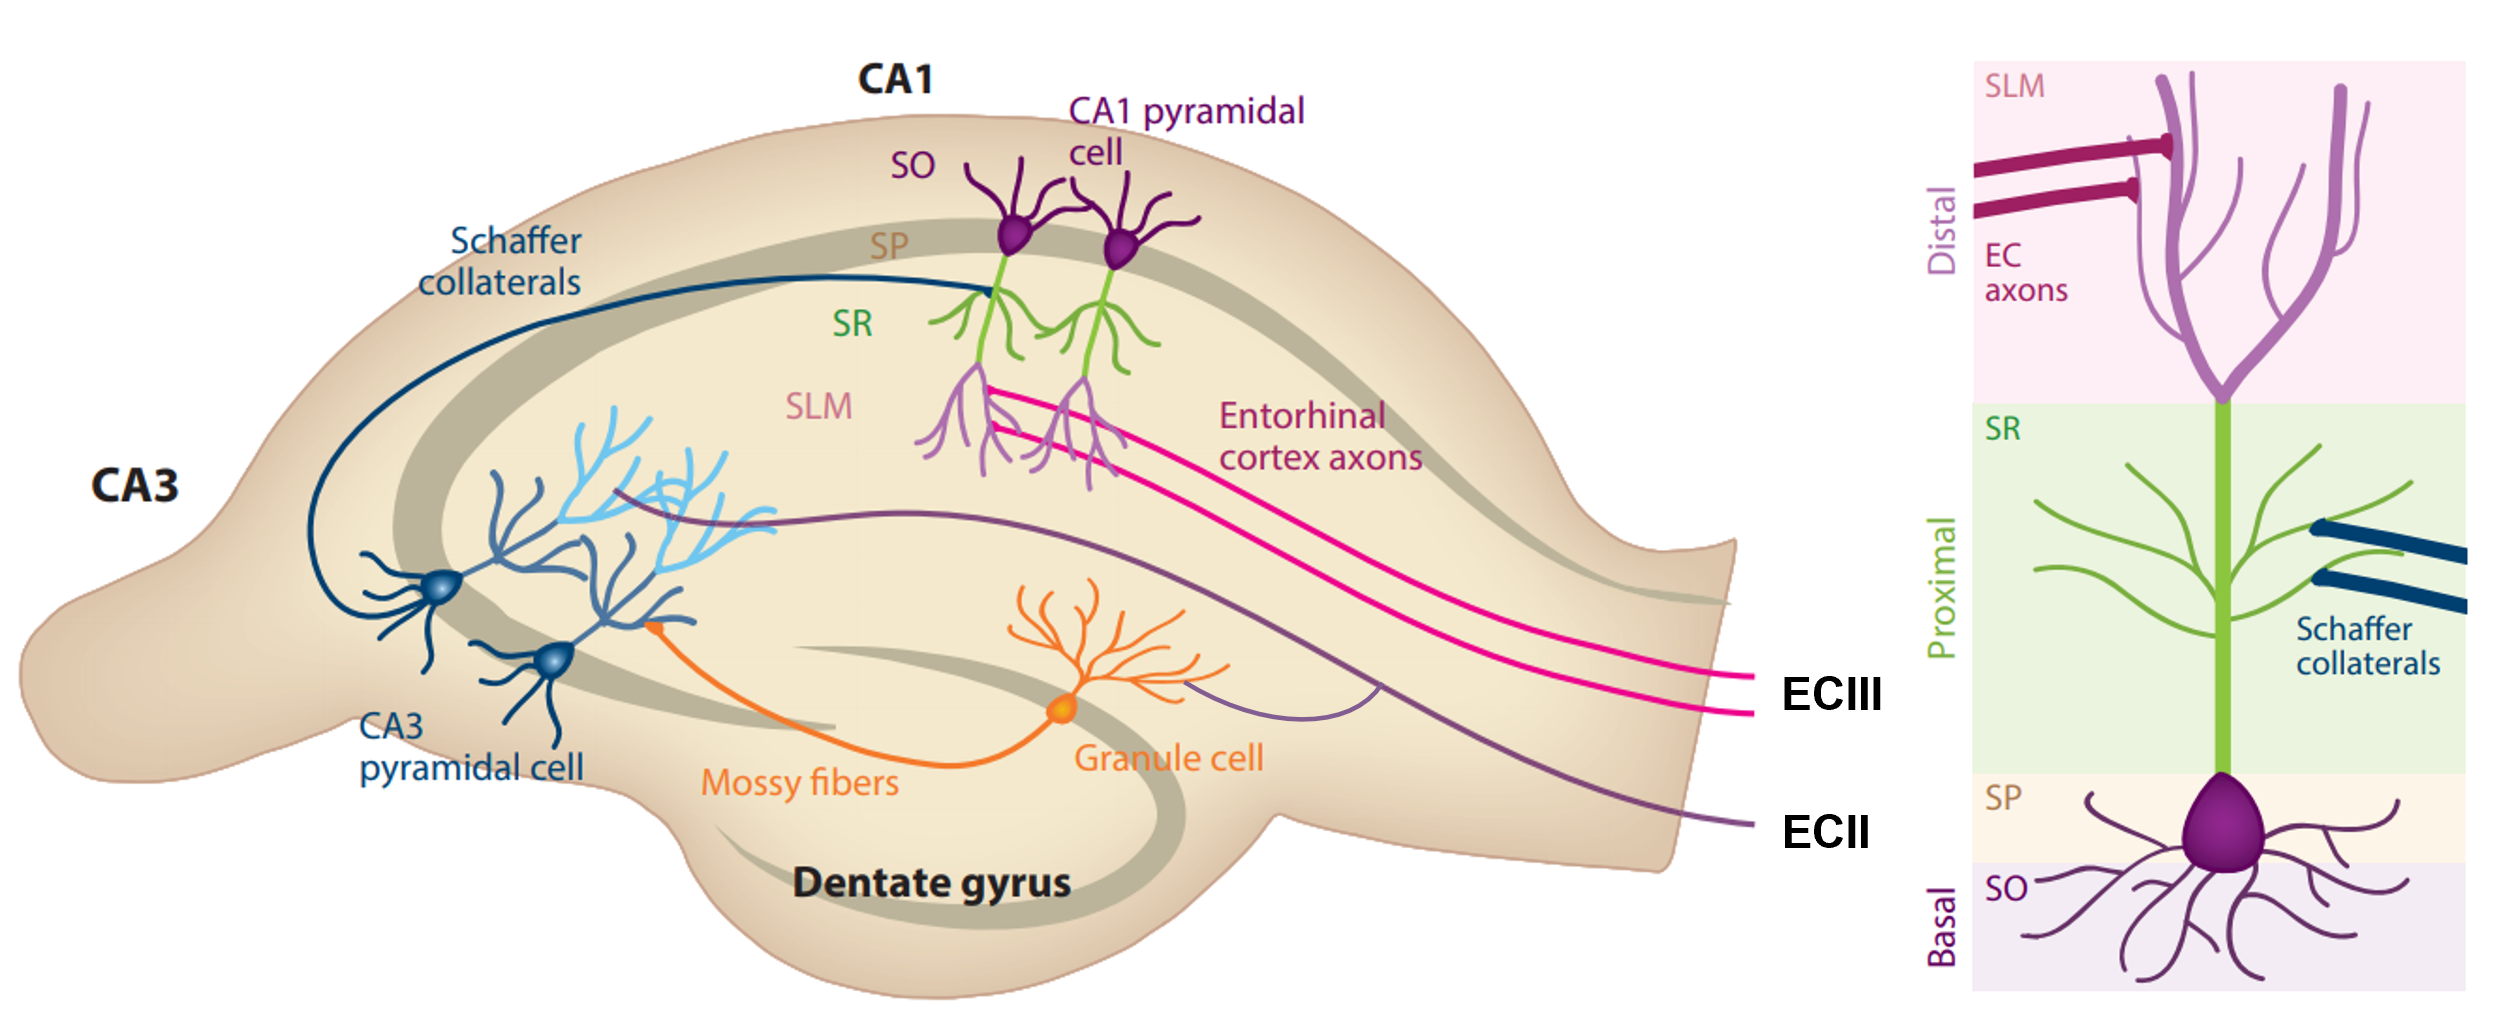
\includegraphics[width=\textwidth]{chapter4/figures/hippocampus-structure.png}
    \caption{\textbf{Laminar organization} of dendritic domains of hippocampal principal neurons: granule cells in DG and pyramidal cells in CA3 and CA1 subregions (right). \textbf{Dendritic domains} of CA1 pyramidal cells include basal and apical dendrites, where the latter is subdivided in proximal and distal dendrites. Excitatory inputs are received from the Schaffer collaterals at proximal dendrites in the SR, while distal dendrites receive excitatory inputs from ECIII (left). Figure adapted from \citep{lefebvre_development_2015}.}
    \label{fig:hippocampus_structure}
\end{figure}

\subsection{Principal cells in CA3 and CA1 subregions}
Hippocampal neuronal circuits comprise populations of relatively homogeneous excitatory neurons, known as principal cells or \textbf{pyramidal cells} (PC), alongside highly diverse inhibitory neurons, termed \textbf{interneurons} (INs).

The distinct layered structure of the hippocampus is a result of the organized arrangement of \textbf{pyramidal cells} \citep{amaral1989three}. Within the CA1 region, the cell bodies of CA1 PCs are located in the \textit{stratum pyramidale}, extending a large-caliber apical dendrite into the \textit{stratum radiatum}, along with fine oblique dendrites.
This apical dendrite then splits within the \textit{stratum lacunosum} to form a tuft in the \textit{stratum moleculare}, collectively known as the \textit{stratum lacunosum-moleculare}. 
Meanwhile, the basal dendrites of CA1 PCs emerge from the cell body and extend into the \textit{stratum oriens}.
The axons of CA1 PCs, originating from either the cell body or a proximal dendrite \citep{thome2014axon}, traverse the \textit{stratum oriens} and project along the alveus, with some axon collaterals branching within the \textit{stratum oriens} to establish recurrent synapses.

Primary afferent inputs into CA1 originate from the Schaffer collaterals in CA3, which synapse in the \textit{stratum radiatum} and \textit{oriens}; temporoammonic axons from ECIII projecting to the \textit{stratum lacunosum-moleculare}; and CA1 recurrent axons that terminate mainly in the \textit{stratum oriens}, often forming synapses with inhibitory neurons \citep{takacs2012extrinsic}.

% Interneurons that primarily receive external inputs are classified as feedforward elements, whereas those that receive local recurrent inputs are regarded as feedback components.
The CA3 subfield shares a remarkably similar structure to CA1, but CA3 PCs exhibit significant morphological differences.
The layering of CA3 resembles CA1, except for the presence of mossy fiber projections originating from DG granule cells, forming a compact bundle in the \textit{stratum lucidum} between the \textit{stratum pyramidale} and \textit{radiatum}.
% Additionally, CA3 PCs establish  associational-commissural collateral projections within the CA3 region, directing the primary synaptic input to the \textit{stratum radiatum} and \textit{stratum oriens}.
Additionally, as a difference of CA1 PCs, CA3 PCs establish high-density recurrent connections between themselves, crucial for pattern completion, a distinguishing feature of the CA3 subfield.
These connections primarily target the stratum radiatum and stratum oriens.
Consequently, inhibitory neurons located in these layers can function as both feedforward and feedback elements, influencing circuit activity in multiple ways.
While CA3 shares many of the IN subtypes in CA1, there are notable differences in IN morphology.
Moreover, the CA3 region also hosts several unique IN subtypes not present in CA1 \citep{tukker2007cell}.
\subsection{GABAergic interneurons in CA3 and CA1 subregions}
Inhibitory interneurons release GABA and are capable of controlling the activity of principal cells and other interneurons, with a large impact on neuronal dynamics. They can regulate neuronal discharge timing, modulate synaptic transmission, and prevent excessive activity.
Although constituting approximately 10-20\% of neurons within specific regions (\textit{i.e.}, CA1, CA3, and DG), interneurons display remarkable diversity in terms of shape, connectivity, and electrical properties, allowing for various classification approaches \citep{petilla2008petilla,somogyi2005defined,klausberger_gabaergic_2009,booker_morphological_2018,tzilivaki_hippocampal_2023}:
\begin{enumerate}
\item Based on postsynaptic targets, leading to three primary classes: \textbf{perisomatic inhibitory} (PI) interneurons, \textbf{dendritic inhibitory} (DI) interneurons, and \textbf{interneuron-specific} (IS) interneurons.
\item Based on morphology, encompassing common types like \textbf{basket} (BC) cells and \textbf{bistratified} (BI) cells.
\item Based on molecular expression, including prevalent markers such as \textbf{parvalbumin} (PV), \textbf{somatostatin} (SOM), \textbf{vasoactive intestinal peptide} (VIP) and \textbf{calcium-binding protein calretinin} (CR).
\item Based on electrophysiological properties, with distinctive classes like \textbf{fast-spiking} (FS), \textbf{regular-spiking} (RS), and \textbf{low-threshold spiking} (LTS) interneurons.
\end{enumerate}
It is important to note that these classification schemes are not mutually exclusive.
An interneuron may belong to multiple categories; for instance, it could be both a PI interneuron and a PV-expressing interneuron.
Moreover, besides these schemes, other classification methods exist, such as grouping interneurons based on developmental origin, yielding non-overlapping categories. \citep{rudy2011three,tzilivaki_hippocampal_2023}.
% \textcolor{blue}{For instance, PV and SOM-expressing interneurons stem from the medial ganglionic eminence (MGE), while serotonin receptor 3a (5HT3AR)-expressing interneurons originate from the caudal ganglionic eminence (CGE).
% (Creo que esto lo podemos omitir).}

Although the same types of interneurons can be found in both CA3 and CA1 subregions, they may differ or possess exclusive types of interneurons.
For example, in CA3, there are some differences in the morphology of \text{oriens-lacunosum moleculare} (OLM) neurons, and mossy fiber-associated interneurons are exclusive to this region.
\begin{figure}[!htb]
    \centering
    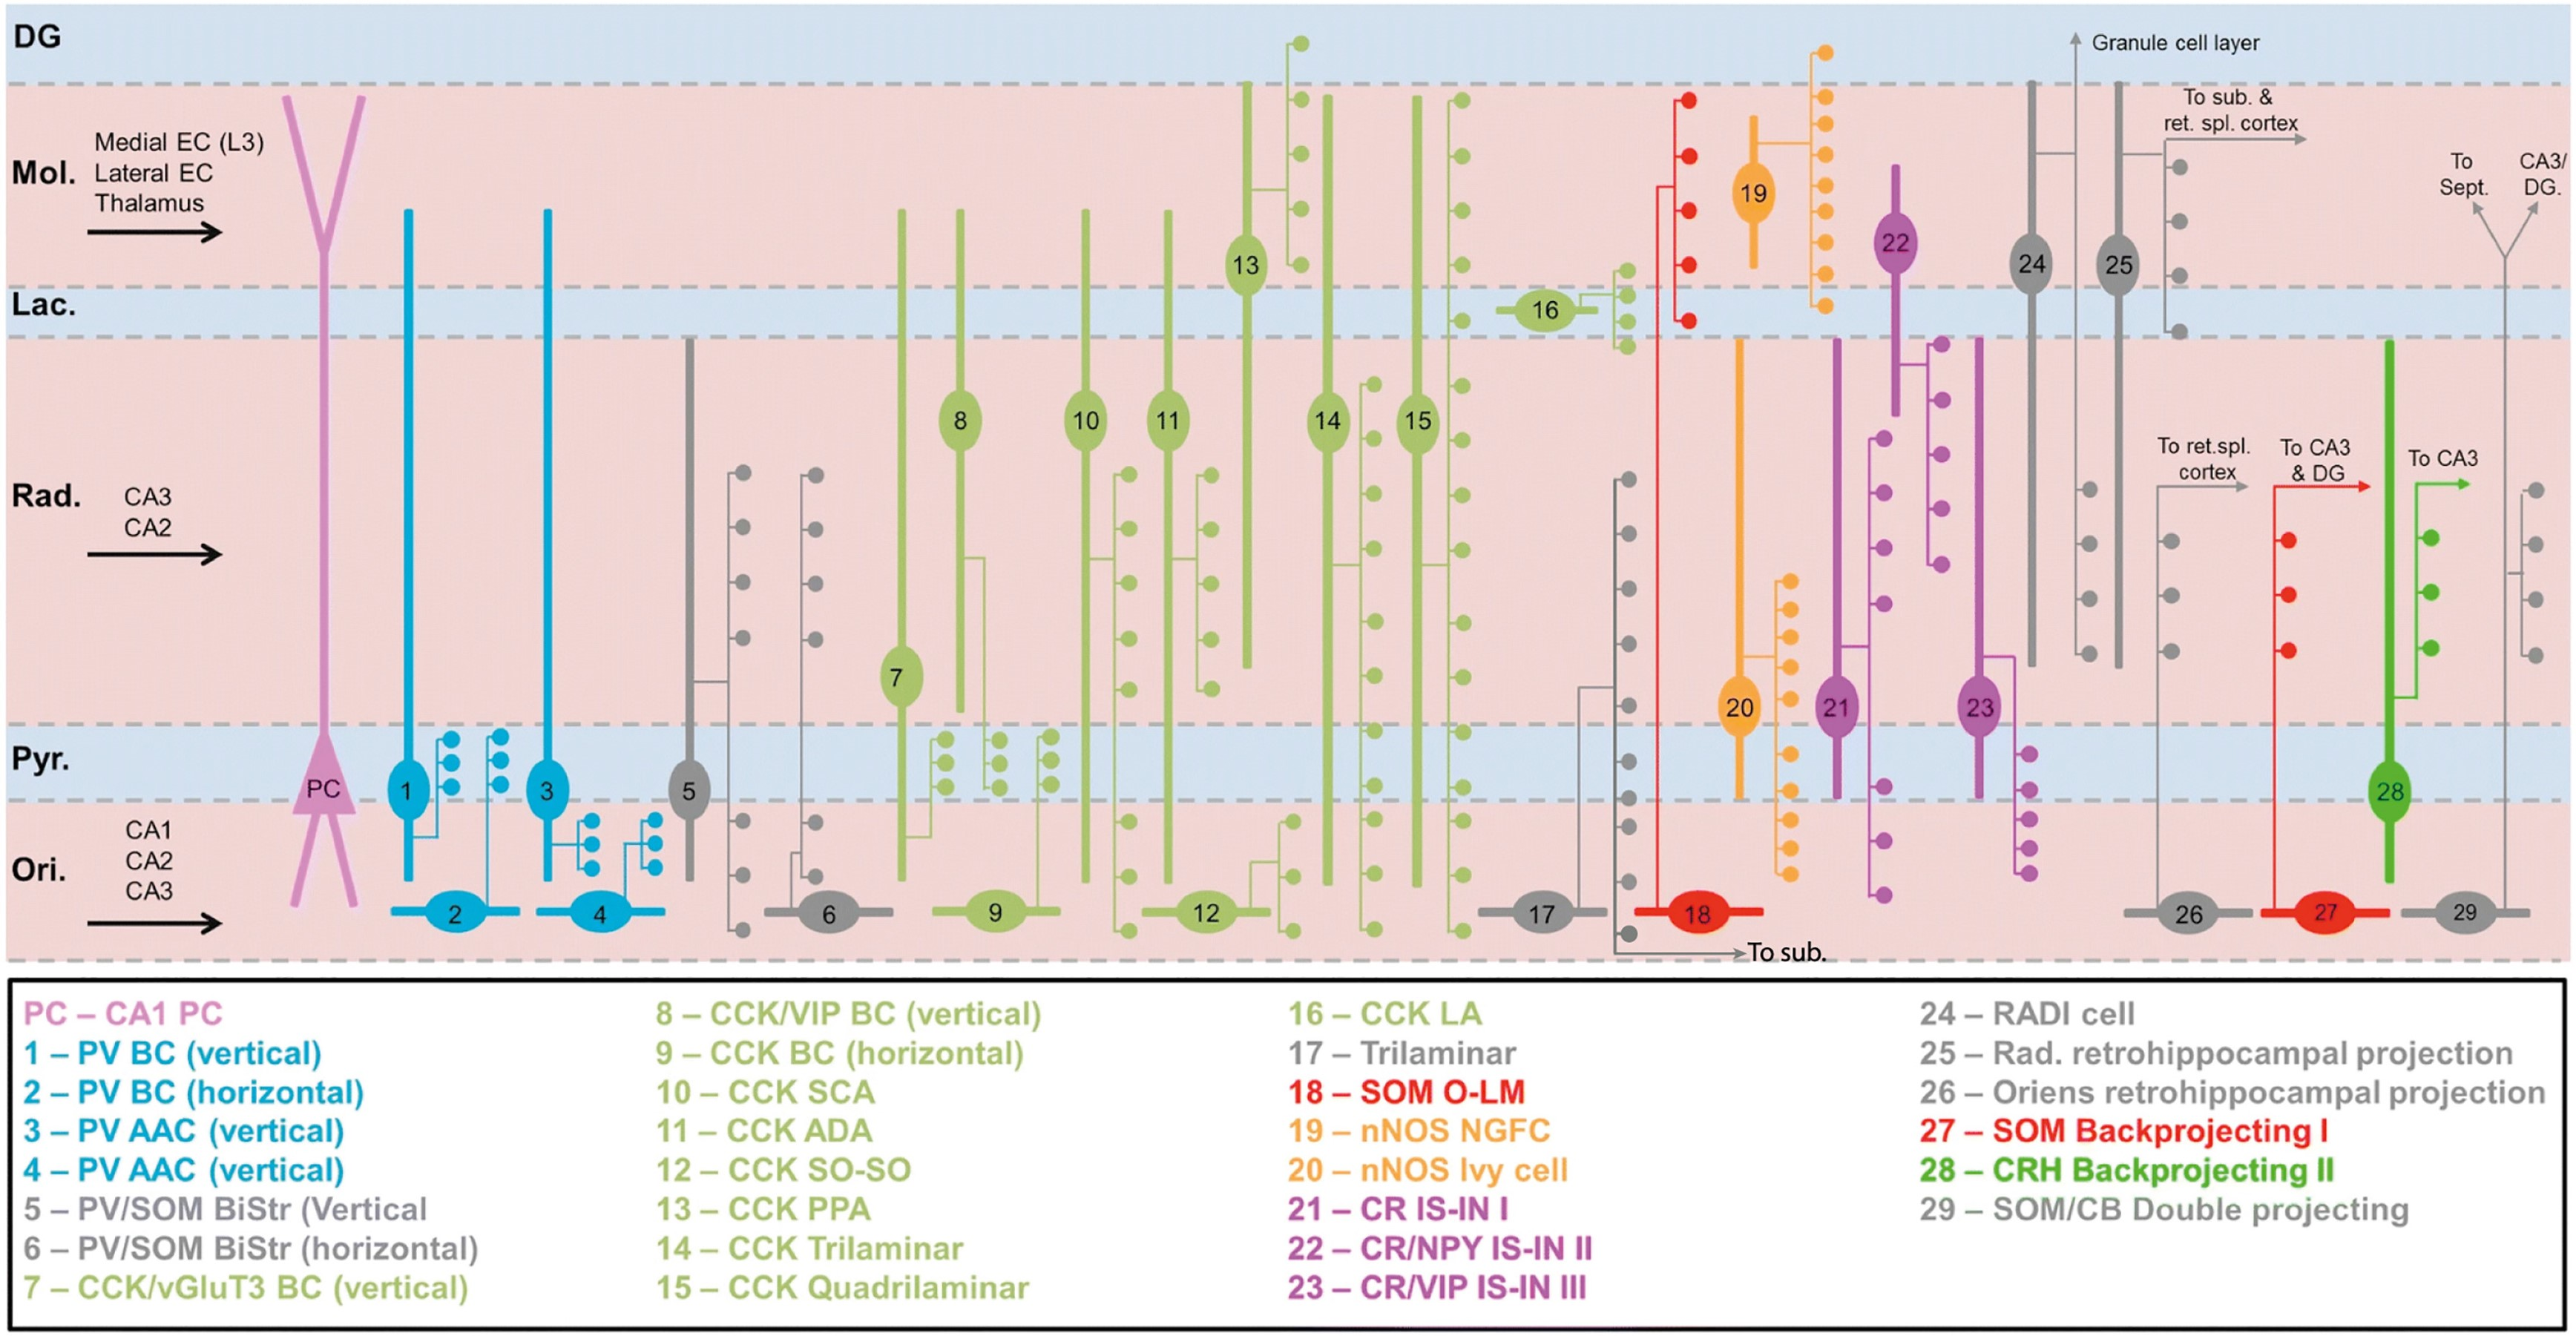
\includegraphics[width=\textwidth]{chapter4/figures/interneuron-diversity-CA1.jpg}
    \caption{\textbf{Interneuron diveristy in hippocampus CA1 subregion}.
    Each interneuron type is depicted with colored dots indicating the locations of axon terminations and thicker lines illustrating their dendritic distribution.
    External inputs are represented by black arrows pointing to the relevant layers. Although there have been reports of additional projections, they are not included in the illustration.
    The pyramidal cell is included to show the dendritic target of interneurons.
     Original figure from \citep{tzilivaki_hippocampal_2023}.}
    \label{fig:interneuron-diversity}
\end{figure}
Therefore, even though what we describe in the subsequent sections is specific to the CA1 subfield, we can extrapolate it to the CA3 subfield.
The vast diversity of internuerons in the CA1 subfield is represented in Figure \ref{fig:interneuron-diversity}.
To describe them, we follow the postsynaptic target classification.

\subsubsection{Perisomatic Inhibitory Interneurons}
The extensively characterized PI interneurons encompass \textbf{basket cells} and \textbf{axo-axonic cells}.
BCs primarily target the somata and proximal dendrites of pyramidal cells, while AACs focus on the axonal initial segment of pyramidal cells.
These PI interneurons have garnered considerable research attention as a result of their prevalence, exerting significant and functionally relevant inhibitory effects. 
Despite constituting around 25\% of known anatomical and neurochemical interneuron subtypes, they account for roughly 50\% of all interneurons, underscoring their crucial role in microcircuit function \citep{booker_morphological_2018}.

\paragraph{Basket Cells}
The most common type of BCs expresses the calcium-binding protein PV, with somata localized in the \textit{stratum pyramidale} or proximal \textit{stratum oriens} and \textit{radiatum}.
PV BCs are typically \textbf{fast-spiking}, exhibiting low membrane resistance and receiving over ten times more excitatory than inhibitory inputs \citep{halasy1996synaptic}.
Another major CA1 BC type expresses the neuropeptide \textbf{cholecystokinin} (CCK). 
CCK BCs, further divided based on co-expression of the neuropeptide VIP, have somata situated in distal \textit{stratum radiatum} \citep{acsady1996different,acsady1996correlated}. 
Unlike PV BCs, CCK BCs receive fewer excitatory than inhibitory inputs and typically exhibit \textit{regular spiking} patterns with adapting trains of action potentials and high input resistance \citep{booker_morphological_2018}.

\paragraph{Axo-Axonic Cells}
AACs express PV with somatic localization similar to that of PV BCs, and they receive strong excitatory inputs from major CA1 inputs, showing a synaptic density comparable to that of PV BCs \citep{buhl1994physiological,papp2013different}.

\subsubsection{Dendritic Inhibitory Interneurons}
DI interneurons constitute a diverse group that predominantly targets the dendritic regions of pyramidal cells and other interneurons.
This varied population \cite{klausberger_gabaergic_2009}, stands out due to their unique dendritic and axonal distributions, distinct neurochemical profiles, and electrophysiological characteristics.
They possess the capacity to selectively restrain PCs through pathway-specific inhibition, targeting either a single layer or extending their axons across multiple layers \citep{melzer2012long}.

\paragraph{Bistratified Cells}
BICs expressing both PV and SOM have somata close to the \textit{stratum pyramidale} and those belonging to CA1 receive robust input from Schaffer collaterals and CA1 PCs.
Their projections span the apical and basal dendrites of CA1 PCs, eliciting smaller and slower IPSCs compared to PV BCs \citep{booker_morphological_2018}.

\paragraph{Oriens/Lacunosum-Moleculare Cells}
SOM-expressing interneurons in the \textit{stratum oriens} are prototypical feedback interneurons in the hippocampus, notably the OLM cells, extensively studied among hippocampal interneuron types.

\paragraph{CCK Cells}
CCK DI cells exhibit substantial morphological diversity in the CA1 region, with several subcategories identified.
Subtypes include \textbf{Schaffer collateral-associated} (SCA) cells with dendrites spanning CA1 layers, heavily innervating \textit{stratum radiatum} and \textit{stratum oriens}, and targeting CA1 PCs.
Other subtypes include CCK DI cells localized in \textit{stratum oriens} inhibiting PC dendrites and CCK \textbf{trilaminar} interneurons projecting to \textit{stratum radiatum}, \textit{stratum oriens}, and \textit{stratum pyramidale} \citep{pawelzik2002physiological}.
% \paragraph{Perforant Path-Associated INs}

\subsubsection{Interneuron-Specific Interneurons}
This group of interneurons primarily inhibits other interneurons, robustly affecting the local microcircuit through dendritic domain inhibition.
They can be divided based on neurochemistry and morphology into three types \citep{tyan_dendritic_2014}: Type I expresses CR but not VIP, primarily found in \textit{stratum oriens}, \textit{pyramidale}, and \textit{radiatum}; Type II co-expresses CR and VIP, typically located in \textit{stratum lacunosum-moleculare}; and Type III expresses CR, VIP, and nitric oxide synthases (nNOS) and is found in \textit{stratum pyramidale} and \textit{radiatum} \citep{tyan_dendritic_2014, booker_morphological_2018}.

\subsubsection{Long-range projecting interneurons}
While GABAergic neurons are mainly associated with local interneurons, there exists a diverse category of \textbf{long-range projecting} (LRP) interneurons.
Three primary projection patterns have been identified, each likely associated with distinct functional roles \citep{jinno2007neuronal,melzer2020diversity}.
The first subgroup is composed of entorhinal cortex and subicular complex-targeting interneurons located in the CA1 region, commonly referred to as \textbf{retrohippocampal-projecting} interneurons.
The second subgroup are interneurons in CA1 known as \textbf{back-projecting} interneurons, characterized by their projections extending \textit{back} to encompass significant portions of CA3 and the dentate gyrus \citep{sik1994inhibitory}.
The third major category among LRP interneurons comprises \textbf{extrahippocampally projecting} interneurons.
This subgroup includes a subset of SOM cells with projections reaching one or more extrahippocampal regions, including the medial septum, medial entorhinal cortex, striatum, and contralateral DG \citep{melzer2012long}.

\subsection{Rhythms in the hippocampus: Theta-gamma cross-frequency coupling}
The hippocampus displays a diverse array of neural oscillations crucial to its functional dynamics.
Among these oscillations are the \textbf{theta} and \textbf{gamma} rhythms, extensively researched in freely moving animals for their pivotal roles in cognitive functions such as memory encoding, retrieval, and spatial navigation \citep{buzsaki_theta_2002,colgin_rhythms_2016}.

The \textbf{theta} rhythm, with a frequency range of 4-12 Hz, is a prominent oscillatory activity within the hippocampus, often linked to exploratory behaviors and memory tasks.
Its generation is primarily attributed to the rhythmic firing of neurons in the medial septum and diagonal band of Broca, influencing hippocampal neuronal activity \citep{buzsaki_theta_2002,buzsaki2006rhythms,mizuseki_theta_2009}.
This rhythm is believed to provide a temporal framework enabling neurons to represent both spatial and non-spatial information, thereby facilitating the temporal organization of neural activity.

In contrast, the \textbf{gamma} rhythm, which oscillates at a higher frequency range of 30-200 Hz, is frequently observed within local field potentials, playing a crucial role in information processing and integration across brain regions \citep{colgin_rhythms_2016}.
These oscillations are categorized into subtypes: \textbf{slow gamma} (30-50 Hz), \textbf{middle gamma} (50-90 Hz), \textbf{fast gamma} (90-150 Hz) and \textbf{ripple oscillations} (150-200 Hz) \citep{mysin_model_2021}.
However, variations may exist depending on different bibliographic source.
The generation of \textbf{gamma} oscillations involves interactions between excitatory pyramidal neurons and inhibitory interneurons within the hippocampal circuits.
The precise timing of \textbf{gamma} oscillations is believed to promote the synchronization of neuronal assemblies, significantly contributing to information processing and transmission \citep{hyafil_neural_2015}.

The interaction between theta and gamma rhythms transcends mere coincidence and represents a structured, functional coupling known as \textbf{cross-frequency coupling} (CFC).
% This concept adds a layer of complexity to the coordination and organization of neuronal activity within the hippocampus, thereby facilitating a deeper comprehension of hippocampal function and its significance in cognition 
This phenomenon reveals intricate relationships between different oscillatory patterns in the brain, providing insights into the coordinated activity of neuronal populations.
By understanding the mechanisms underlying CFC, we can gain deeper insights into the complex dynamics of hippocampal function and its role in cognitive processes \citep{jirsa_cross-frequency_2013,hyafil_neural_2015}.

Experimental and theoretical studies suggested that episodic memory consolidation involves two steps, encoding and retrieval, ocurring at different phases of the CA1 subregion theta oscillation.
% , as depicted in Figure \ref{fig:encoding_retreival}.
During the encoding step, input from the ECIII reaches the CA1 subregion, whereas during retrieval, output from the CA3 subregion to CA1 via the Schaffer collaterals is involved \citep{judge_theta_2004,ketz_theta_2013}.
The transmission of information between these regions, including the DG subregion, is proposed to take place during \textbf{gamma} oscillations of varying frequencies organized within the phase of the \textbf{theta} rhythm.
% \begin{figure}[htb]
%     \centering
%     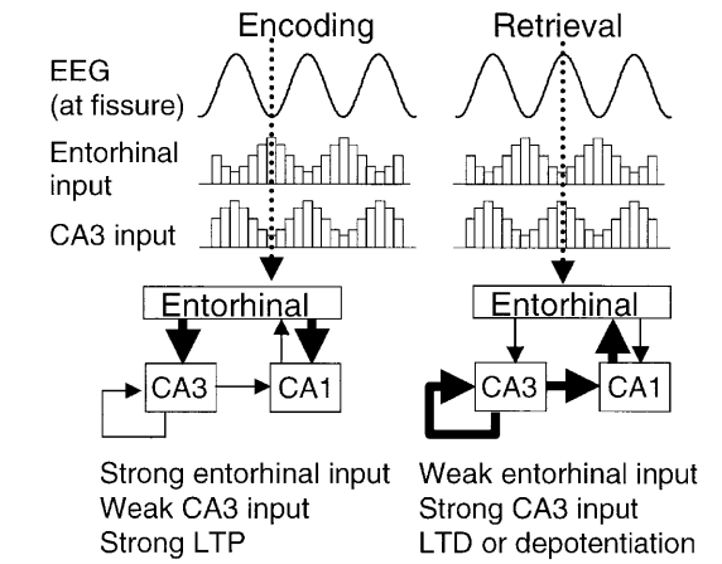
\includegraphics[width=0.8\textwidth]{chapter4/figures/encoding-retreival.png}
%     \caption{\textbf{Memory cycle scheme.}
%     Left: \textbf{Encoding}. 
%     At the peak of the local CA1 theta, synaptic currents arriving from EC are strong, whereas those from CA3 are weak.
%     The latter exhibit strong long-term potentiation (LTP) capacity, allowing effective encoding of new associations while preventing interference from prior ones.
%     Right: \textbf{Retrieval}. 
%     On the contrary, at the troughs of CA1 theta, synaptic currents arriving from are weak where those from CA3 are strong.
%     In this phase, the CA3 inputs undergo potentiation rather than LTP, allowing for effective retrieval of prior associations. 
%     Original figure from \citep{judge_theta_2004}.}
%     \label{fig:encoding_retreival}
% \end{figure}
However, it is well-established that the hippocampus generates different theta rhythms from various layers, necessitating the consideration of theta-gamma interactions within the context of multiple rhythm generators \citep{buzsaki_theta_2002,lopez-madrona_different_2020}.
Lopez-Madrona et al. \citep{lopez-madrona_different_2020} conducted an insightful analysis in this regard, examining the interaction of three distinct and independent theta oscillations along with their corresponding gamma oscillations.
One theta oscillation was identified in the \textit{str. radiatum} in CA1, where CA3 pyramidal cells project to CA1 pyramidal cells via Schaffer collaterals.
The second oscillation was localized in the \textit{str. lacunosum moleculare}, where ECIII pyramidal cells provide excitatory projections.
Lastly, the third oscillation was situated in the mid-molecular layer of the DG, where granule cells receive inputs from ECII.
Their findings revealed that these layer-specific theta oscillations can dynamically couple and decouple, suggesting a mechanism for integrating or segregating computations.
And likewise, the interaction of gamma activity with theta was to be considered independently for each theta framework.
This finding contrasts with previous models that concentrated solely on a single theta cycle \citep{lopes2018parsing,dvorak2018control,zhang2019sub}.
This suggets parallel processing in cell assemblies that receive information from different theta frameworks.
A decrease in coherence between theta oscillations separates cognitive processes (\textit{i.e.}, retrieval from encoding), while an increase in coherence couples them, aiding the integration of information in CA1 neurons and downstream regions.
\begin{figure}[!htb]
    \centering
    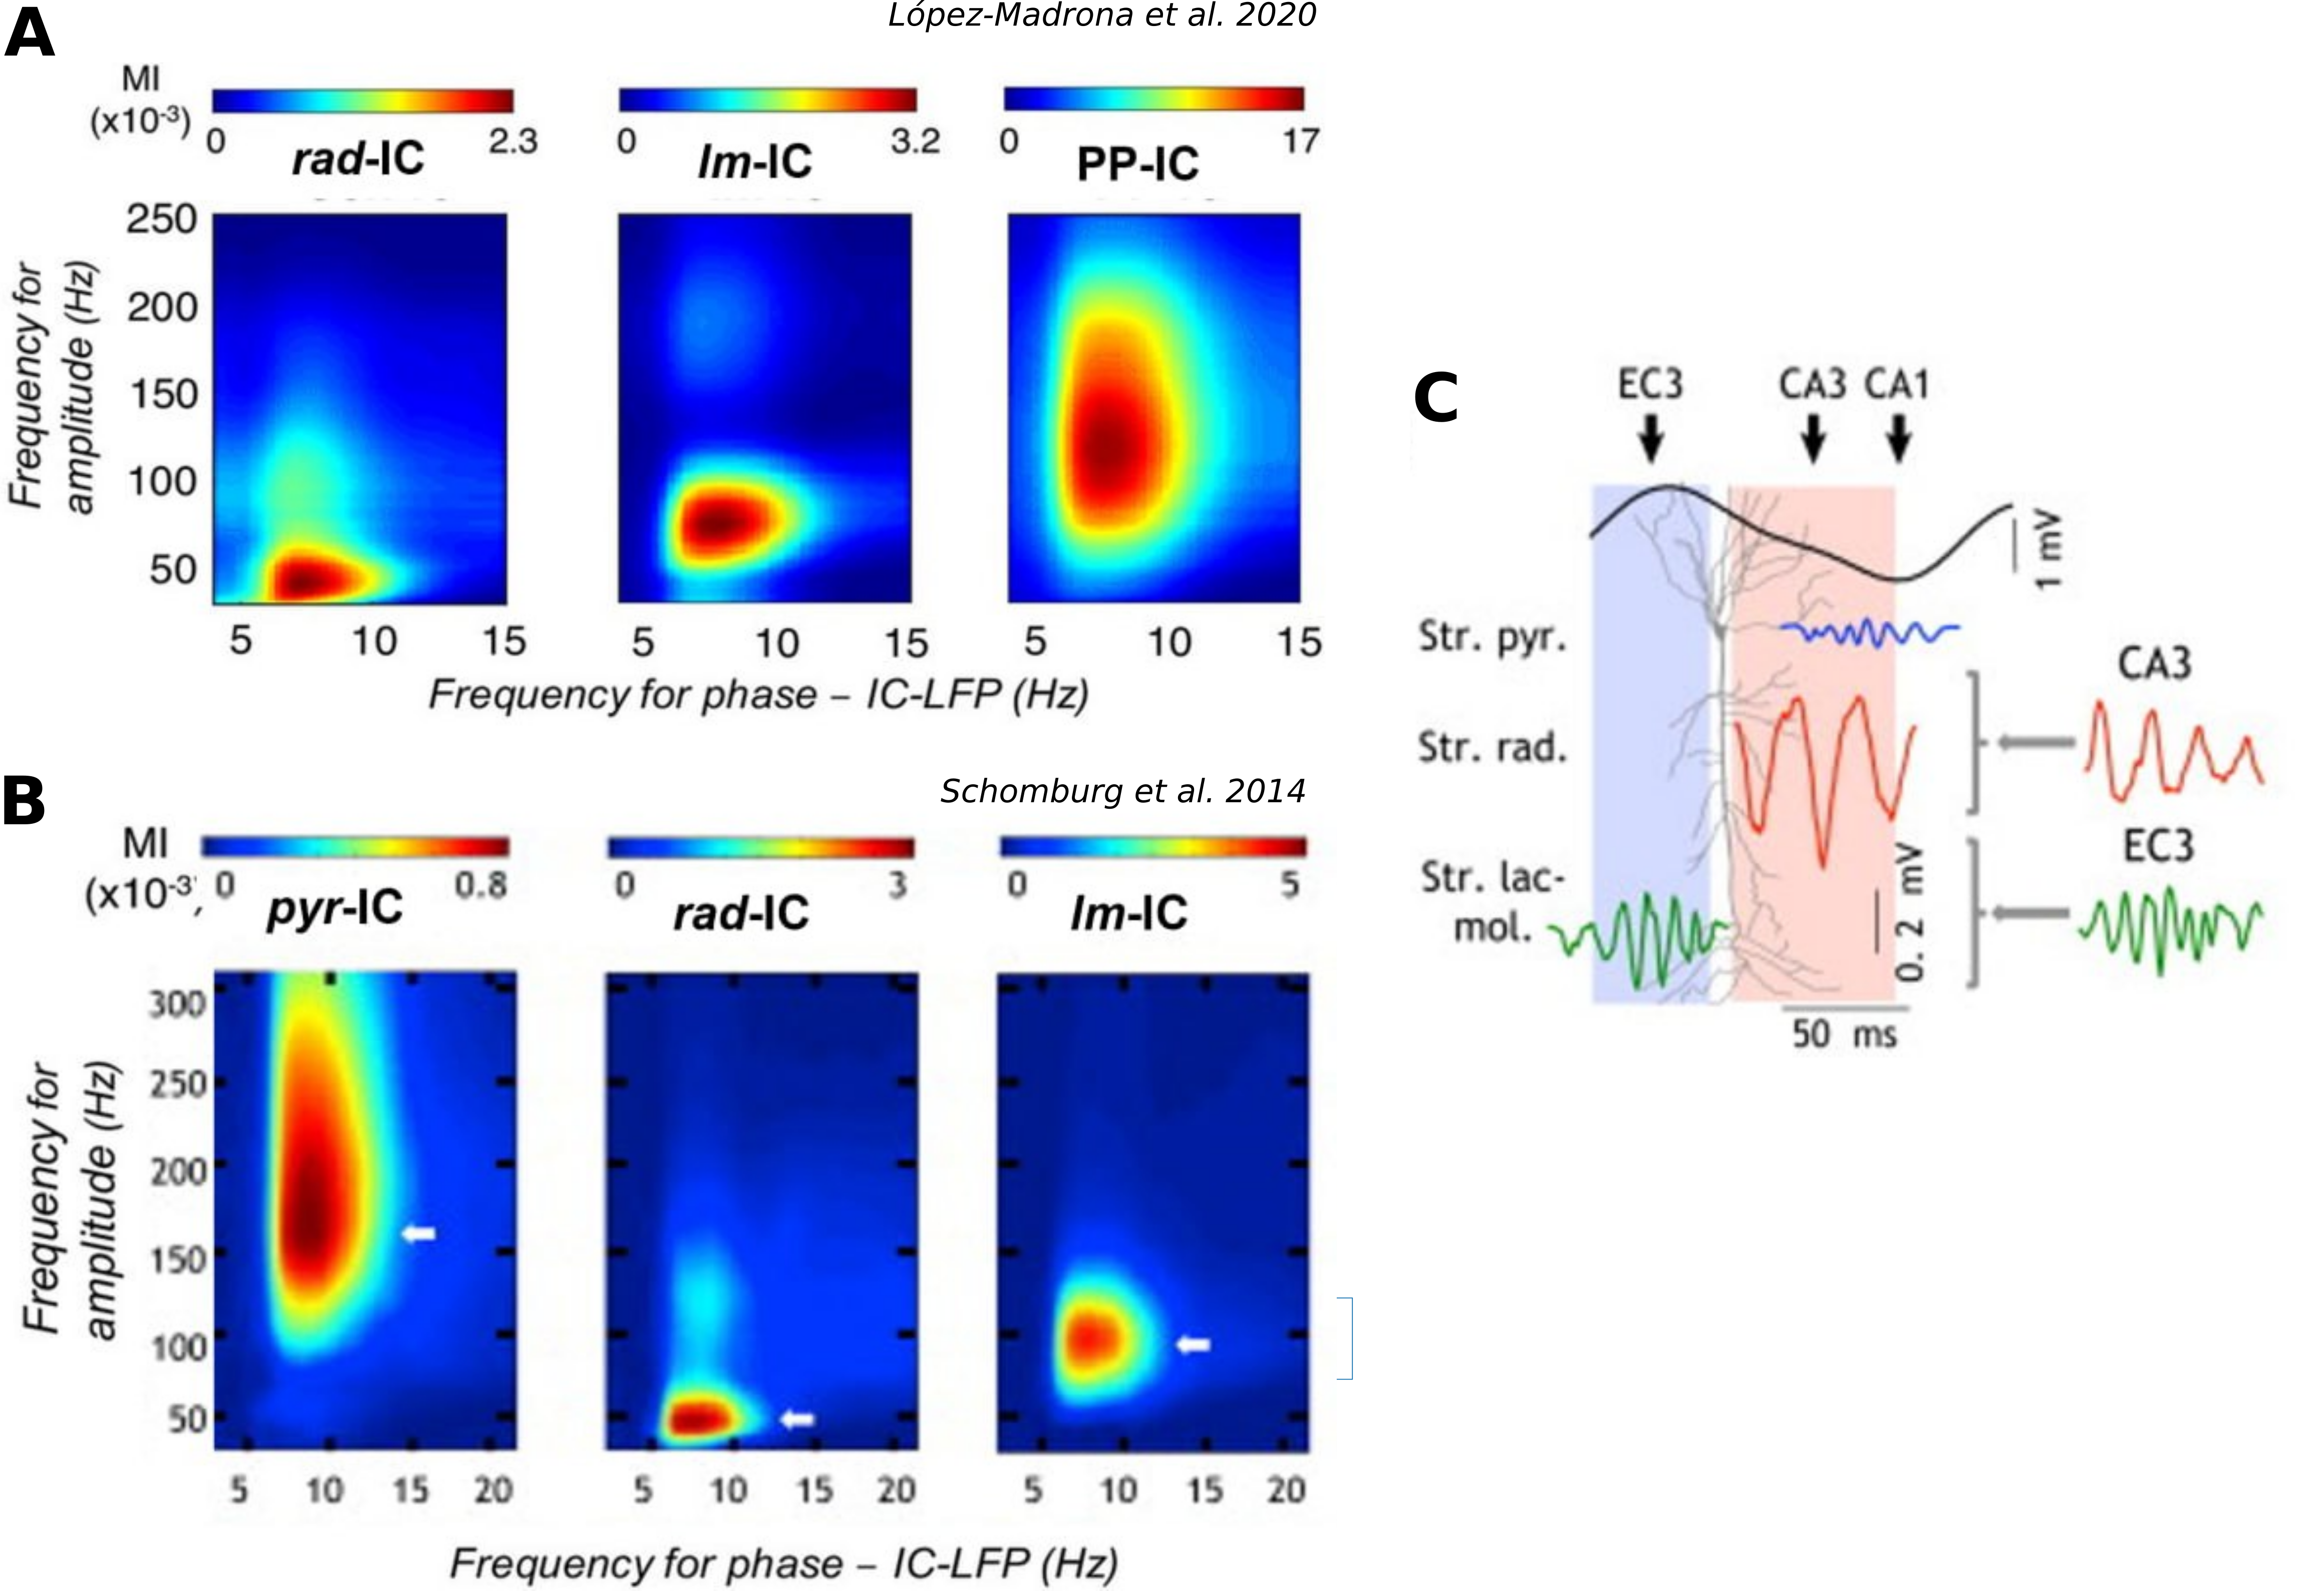
\includegraphics[width=\textwidth]{chapter4/figures/modulation-index-examples.png}
    \caption{\textbf{Cross-frequency coupling strength, measured by the modulation index, between gamma and the corresponding pathway-specific thetas of the independent component of the LFPs (ICs)}.
    Panel A shows the results from experiments by Lopez-Madrona et al. \citep{lopez-madrona_different_2020} how independent components localized in the \textit{stratum radiatum} (\textit{rad}-IC), \textit{stratum lacunosum moleculare} (\textit{lm}-IC), and hilus (PP-IC).
    Panel B shows the results from Schomburg \textit{et al.} \citep{schomburg_theta_2014}, where independent components are localized in the \textit{stratum pyramidale} (\textit{pyr}-IC), \textit{stratum radiatum} (\textit{rad}-IC), and \textit{lacunosum moleculare} (\textit{lm}-IC).
    Each independent component exhibits coupling with different gamma subbands.
    Consistent findings are observed across both experiments in the coincident ICs.
    Panel C shows a schematics of the CA1 pyramidal cell reflects the prominence of each gamma subband per stratum and their preference in the theta oscillation of the \textit{stratum pyramidale}.}
    \label{fig:modulation-index-IC}
\end{figure}
Figure \ref{fig:modulation-index-IC} shows the cross-frequency coupling strength, measured by the modulation index (which will be described in the next section) between the corresponding theta and gamma oscillations associated to each layer mentioned.

In addition, each gamma band is associated with different phases of the theta cycle, as schematically shown in the same Figure \ref{fig:modulation-index-IC}.
\textbf{Slow gamma} activity predominates during the descending phase of the theta rhythm in the CA1 pyramidal layer, primarily driven by inputs from the Schaffer collaterals \citep{colgin_frequency_2009, belluscio_cross-frequency_2012, fernandez-ruiz_entorhinal-ca3_2017, mysin_model_2021}.
\textbf{Middle gamma} oscillations are believed to result from inputs originating in the ECIII via the perforant path \citep{lisman_how_2017, mysin_model_2021}.
In contrast, fast \textbf{gamma oscillations} coincide with the troughs of the theta phase, corresponding to maximal firing rates of CA1 pyramidal cells \citep{somogyi_temporal_2014, fernandez-ruiz_entorhinal-ca3_2017,schomburg_theta_2014}.
\textbf{Ripple oscillations} are thought to arise from the rapid synchronization of principal cells in the dentate gyrus (DG) and CA3, driven by robust self-excitation, and subsequently propagate to CA1 \citep{nakashiba2009hippocampal}.

Abnormalities in CFC patterns have been noted in individuals affected by diverse medical conditions, providing insight into potential underlying neural dysfunctions associated with these disorders.
Studies have consistently highlighted altered CFC patterns in patients with Parkinson's disease, Alzheimer's disease, schizophrenia, and other mental health disorders, including anxiety \citep{uhlhaas_neural_2006, wang2017enhanced, abubaker_working_2021, yakubov_cross-frequency_2022, bayraktaroglu_abnormal_2023}.
These irregular CFC patterns can significantly impact the coordination and communication between different brain regions, potentially contributing to the cognitive and behavioral symptoms observed in these conditions.
For instance, in Parkinson's and Alzheimer's diseases, the atypical CFC patterns might disrupt inter-regional communication, leading to cognitive decline and memory impairments \citep{yakubov_cross-frequency_2022, bayraktaroglu_abnormal_2023}.

\subsubsection{Mechanisms of the Cross-frequency coupling}
From a theoretical perspective, diverse modes underlying cross-frequency coupling have been proposed, as illustrated in Figure \ref{fig:CFC-types}: \textbf{phase-amplitude coupling} (PAC), \textbf{amplitude-amplitude coupling} (AAC), \textbf{phase-phase coupling} (PPC), and \textbf{phase-frequency coupling} (PFC).

In AAC, changes in the amplitude of higher frequency oscillations correspond to alterations in the amplitude of lower frequency bands.
Conversely, PPC involves synchronization of oscillations at different frequencies in phase, maintaining a consistent phase relationship. 
PFC modulates the excitability of a fast frequency, involving a fast frequency modulation.
\begin{figure}[!htb]
    \centering
    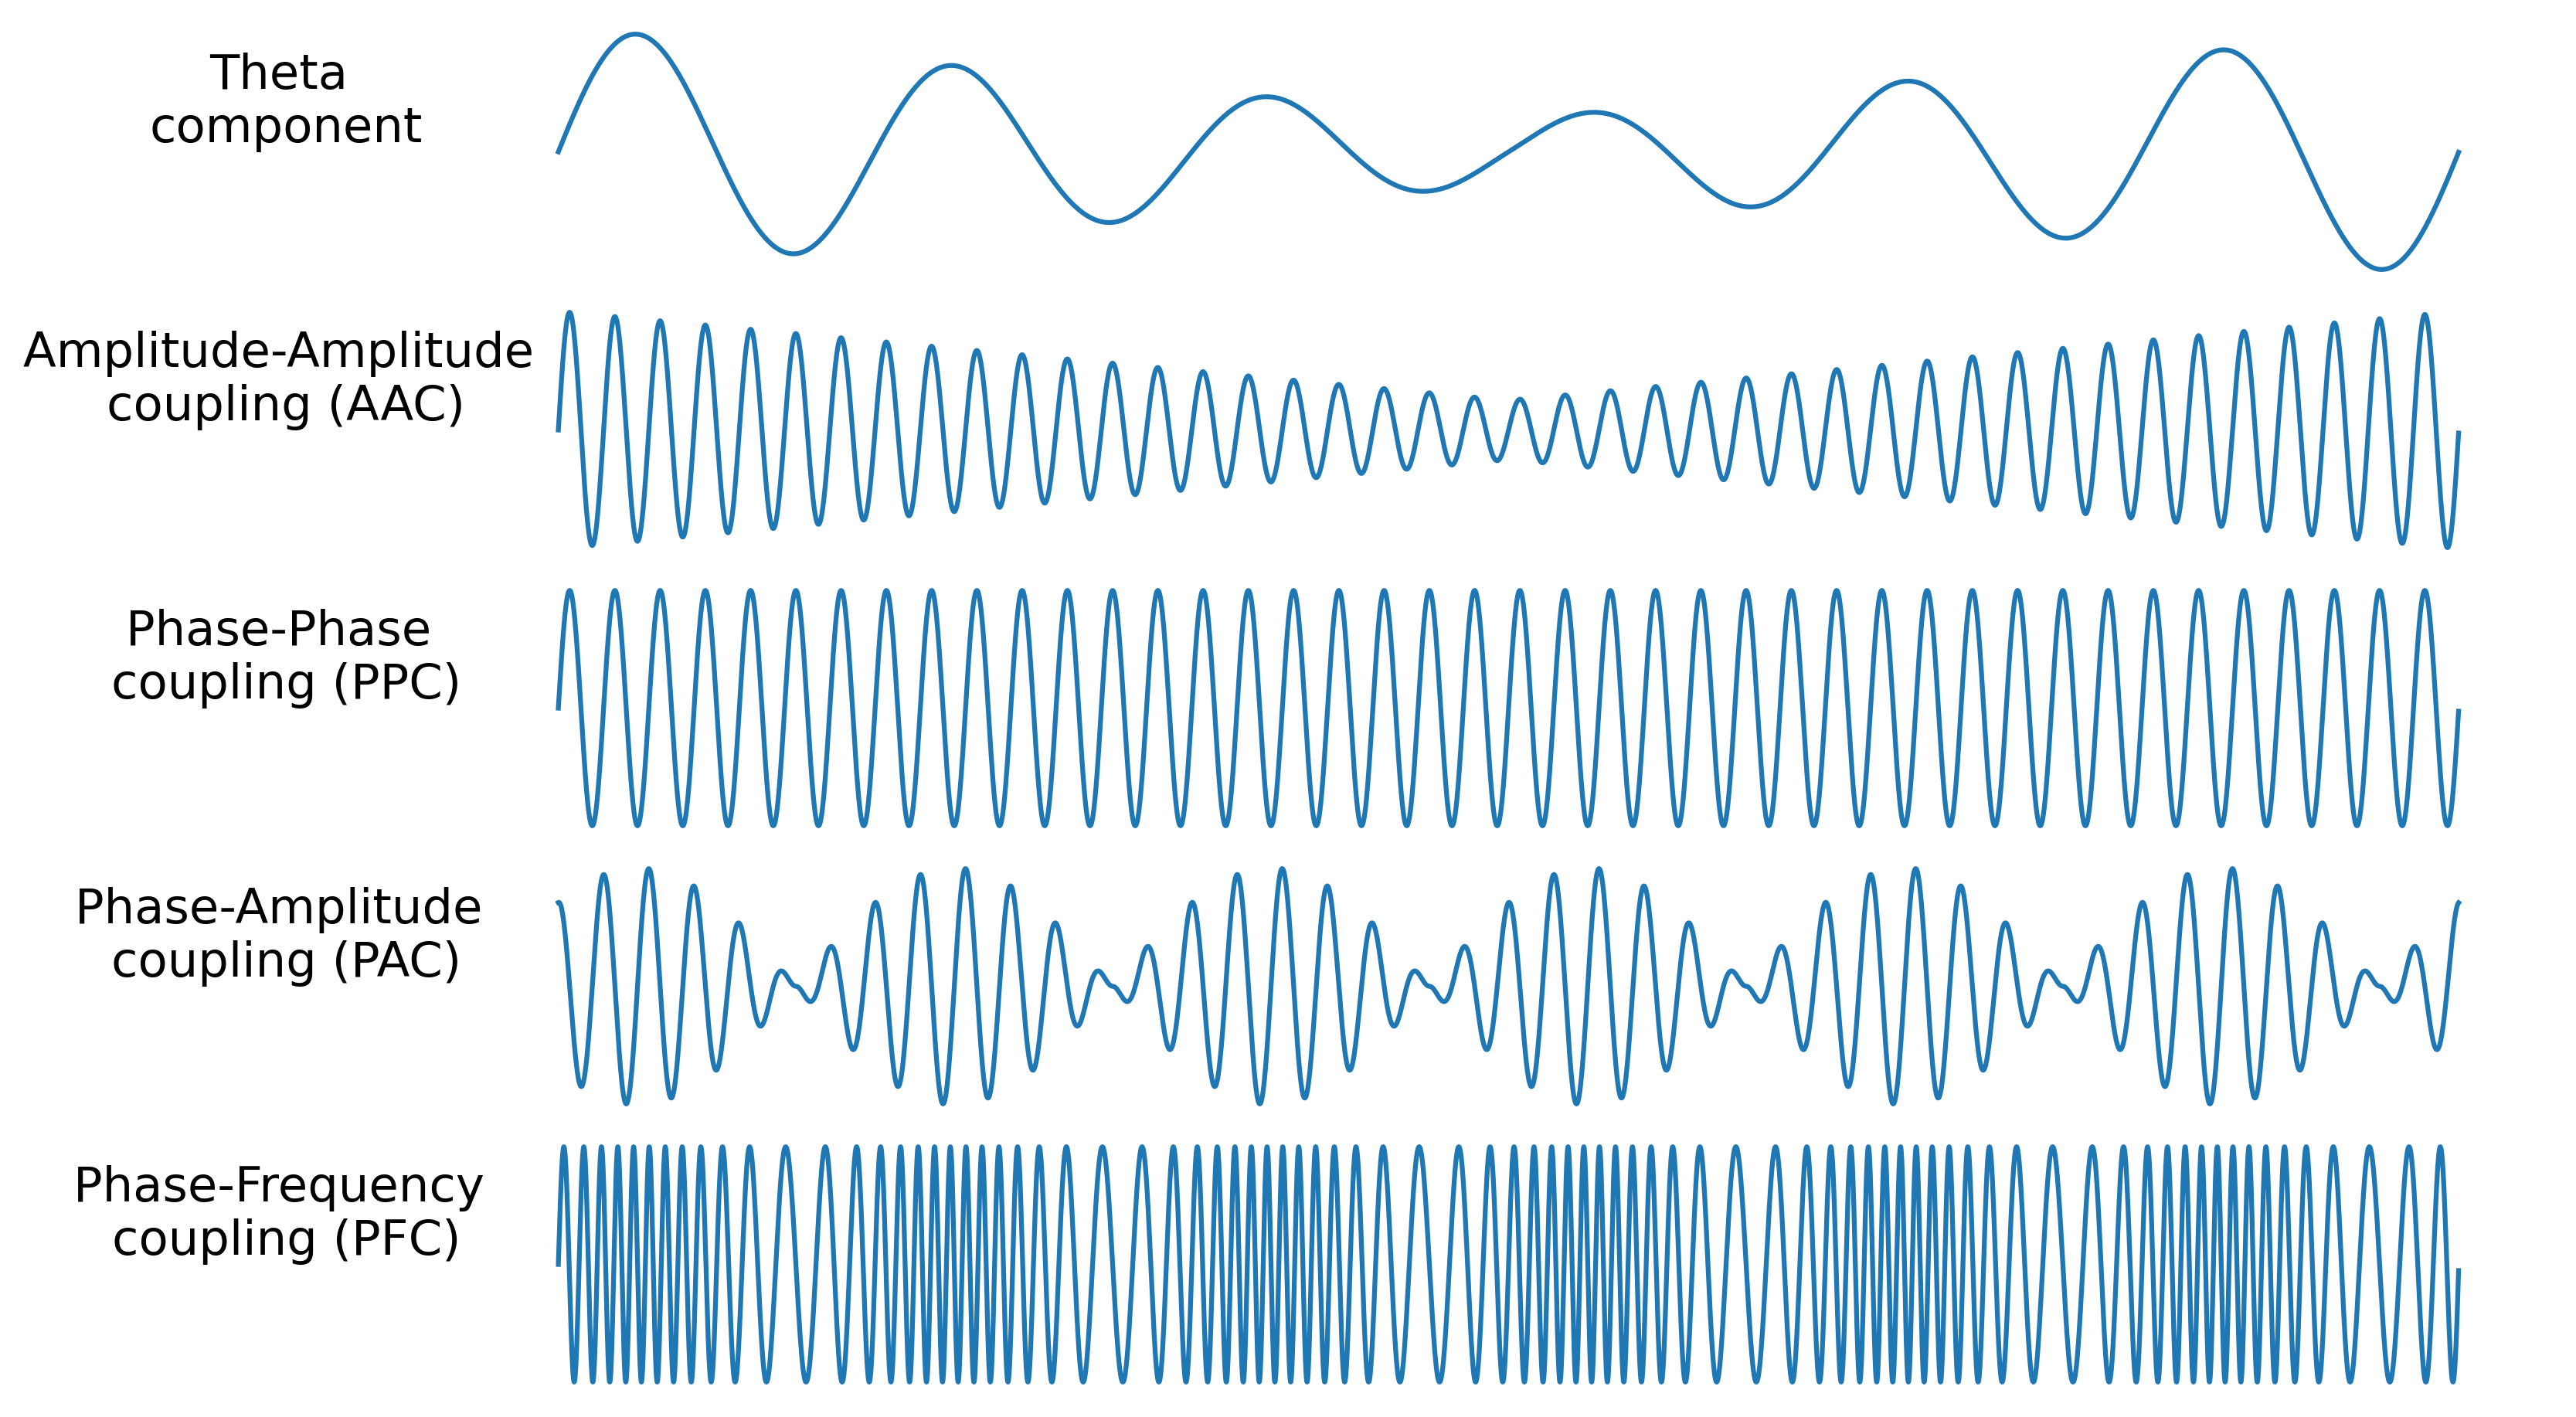
\includegraphics[width=\textwidth]{chapter4/figures/CFC-schematics.png}
    \caption{\textbf{Different modes of cross-frequency coupling from a theoretical point of view}.} 
    % Figure adapted from \citep{muller2022neural}.}
    \label{fig:CFC-types}
\end{figure}
However, PAC is the most commonly observed form of CFC in the brain, where high-frequency oscillation amplitudes are influenced by the phases of low-frequency oscillations.
This type of CFC has been identified in the hippocampus, entorhinal and prefrontal cortices, as well as distributed cortical areas. 
It has been proposed to play a crucial role in sequence coding, inter-regional communication, and integration of signals from various sensory modalities.
Yet, the functional role of AAC remains unclear, and no established biological significance has been attributed to PFC as of yet \citep{canolty_high_2006, jirsa_cross-frequency_2013, hyafil_neural_2015, sotero2016topology, siebenhuhner2020genuine, siems_dissociated_2020}.
Theoretical exploration of CFC, especially between \textbf{slow gamma} and \textbf{theta rhythms}, has been extensively covered in the literature, spanning from detailed biological descriptions to more abstract models \citep{cutsuridis_hippocampal_2018}.
A simplified model frequently considered involves two primary interneuron types: \textbf{fast-spiking PV basket} cells and \textbf{OLM} cells.

The mechanisms generating gamma rhythms, whether observed \textit{in vivo} or \textit{in vitro}, exhibit variability.
\textit{In vitro}, \textbf{slow gamma} frequencies can stem from at least three distinct mechanisms: \textbf{interneuronal network gamma} (ING), \textbf{pyramidal-interneuronal network gamma} (PING), and \textbf{persistent gamma} (PG).
In the ING mechanism, gamma frequencies emerge from the interneuron recurrent feedback inhibition that blocks the effects of AMPA synapses.
Conversely, PING arises from interactions between pyramidal and interneuron populations, wherein both populations fire near or at the population frequency.
\textbf{Persistent gamma}, induced pharmacologically and persisting for several hours, reflects a scenario where pyramidal cells sparsely spikes at low rates (< 5 Hz) while GABAergic interneurons fire close to the population frequency oscillation.
In all three mechanisms, the population frequency is reliant on the decay time constant of GABA$_{\text{A}}$ receptors \citep{traub1996analysis, borgers_effects_2005}.

At present, theoretical models explaining the generation mechanisms of \textbf{middle gamma}, \textbf{fast gamma}, and \textbf{ripple oscillations} have yet to be fully established, although some network models have been proposed to simulate their generation \citep{taxidis2012modeling,jahnke2015unified,omura2015lognormal}.
\paragraph{PING mechanism}
In the PING mechanism, a cycle starts as pyramidal cells receive robust input, inducing them to spike.
These pyramidal neurons project widely onto interneurons, stimulating them to fire and consequently inhibiting further activity of both pyramidal cells and the interneurons they target. 
Pyramidal cells can generate spikes only after the inhibition has decayed sufficiently, aligning their firing close to the onset of the subsequent cycle \citep{jaeger_hippocampal_2013}.

Computational models emphasize the significance of pyramidal cell projections to interneurons in generating oscillations.
Theses oscillations persist even in scenarios where there is no direct stimulation of interneurons or interneuron connections are severed, as long as interneurons receive sufficient input from pyramidal cells.
The frequency of oscillations is influenced by several factors, including the delay between interneuron and pyramidal cell spikes, the time taken for pyramidal cells to overcome inhibition, and the modulation of GABAergic synapse strength.
However, the decay time of GABAergic synapses stands out as the primary determinant of oscillation frequency.
Therefore, populations of interneurons slower and faster synpatic dynamics give rise to different gamma-frequency oscillations \citep{Tort2007}.
Assuming, excitatory neurons as type I, the PING mechanism works if the following conditions are hold \citep{cutsuridis_hippocampal_2018}:
(i) the excitatory cells receive a driver external input, independently of any synaptic input, at or above the gamma frequency, (ii) excitatory synapses are short and strong enough to make inhibitory cells spike, (iii) inhibitory cells spike oinly in response to excitatory cells, and (iv) the inhibitory synpases are strong enough to  facilitate synchronization between the excitatory and inhibitory populations.
The presence of noise and/or heterogeneity makes the analysis of the PING more complicated.
The formation of a coherent gamma rhythm depends on the number of projections that every neuron receive from the opposite population, which is independent of the size of the network.
On the other hand, inhibitory cells synchronize more tightly than the excitatory population \citep{cutsuridis_hippocampal_2018,Wang1996,kopell2002mechanisms}.
\clearpage
\begin{figure}[!htb]
    \centering
    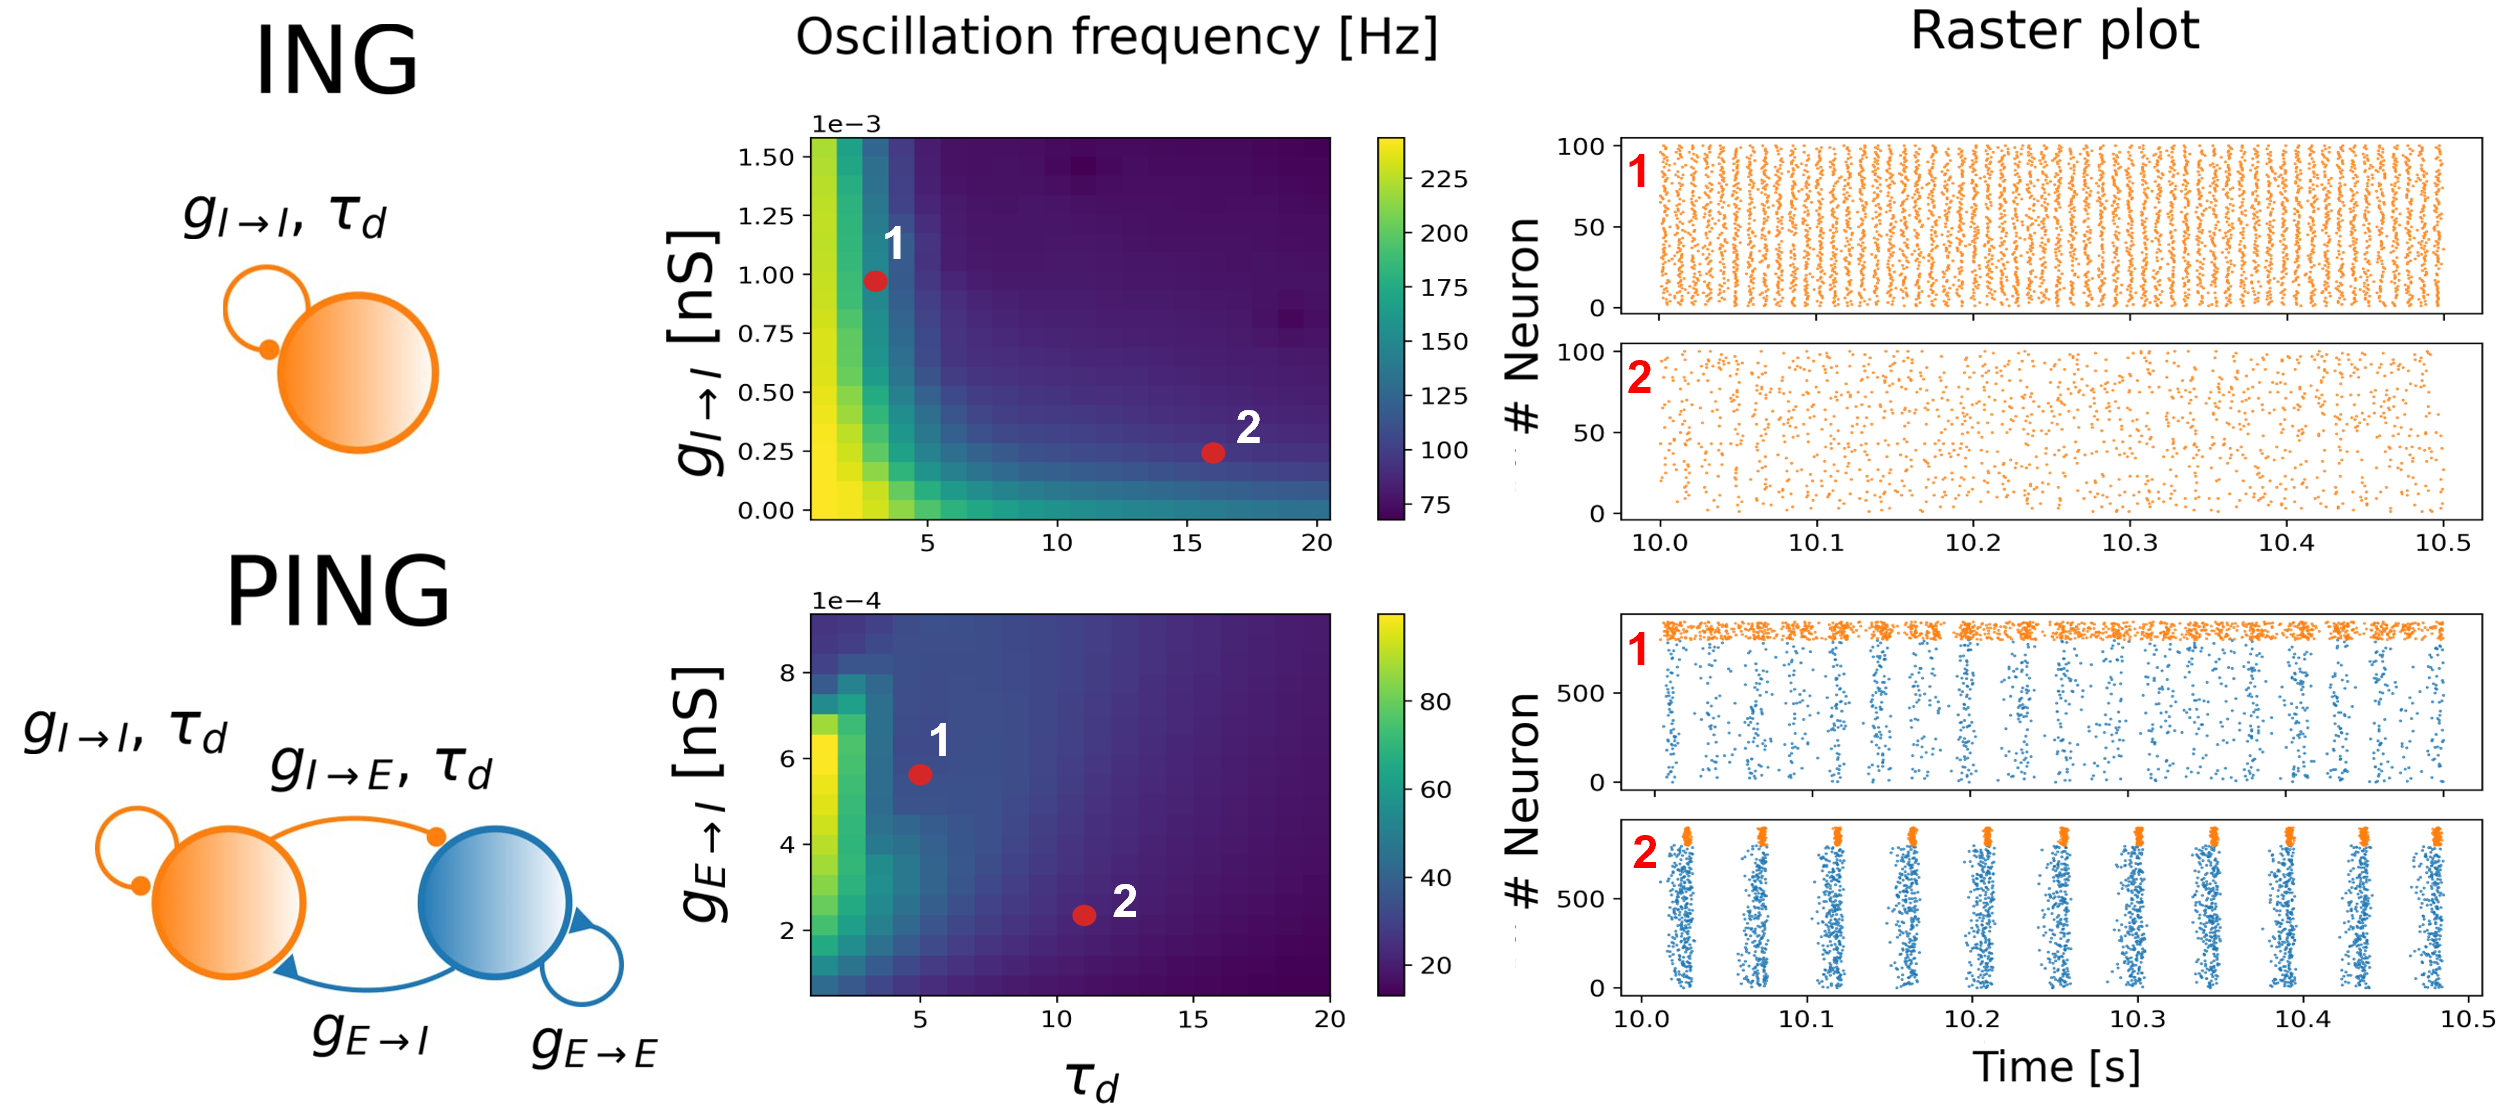
\includegraphics[width=\textwidth]{chapter4/figures/PING_and_ING.png}
    \caption{\textbf{ING and PING mechanisms.}
    Emergent oscillation frequencies in the ING and PING mechanisms.
    For the ING mechanism, we depict the frequency as a function of the conductance and the time decay constant of the GABAergic synapses.
    For the PING mechanism, we illustrate the frequency as a function of the conductance of AMPA projections to the inhibitory cells and the time-decay constant of GABAergic synapses.
    Two raster plots are provided for each mechanism, representing different dynamics.
    To compute them, we used the pyramidal cells and basket cells of our model.}
    \label{fig:PING-mechanim}
\end{figure}

\paragraph{ING mechanism}
ING mechanism represents a fundamental mode of gamma rhythm generation that functions within an interconnected network of interneurons, operating independently of principal cells.
When these interneurons receive a drive, they depolarize and spike at high rates.
This activity results in the inhibition of downstream neurons, causing a delay in their firing.
Given the divergence in neuronal projections, where each neuron form connections to multiple downstream neurons, the inhibitory effect of a single spike can influence a segment of the neuron population. 
Simultaneous spiking by multiple neurons leads to synchronized inhibition among their collective target neurons.
This synchronized inhibition increases the probability of subsequent synchronized spiking among the targeted neurons, promoting the propagation of synchrony throughout the network and giving rise to gamma oscillations \citep{jaeger_hippocampal_2013,cutsuridis_computational_2015}.

The ING mechanism has been extensively explored through computational models, such as the Wang-Buzsáki model \citep{Wang1996}. 
In this model, every neuron connects to every other neuron, exhibiting all-to-all connectivity. 
Upon depolarization of interneurons, the model rapidly demonstrates oscillations in the lower gamma range.
Even when the all-to-all connectivity is replaced with a sparser, random connectivity matrix, synchrony persists as long as sufficient convergent inhibition exists.
The Wang-Buzsáki model illustrates the ING mechanism in its fundamental form, indicating that gamma oscillation generation via ING requires specific conditions \citep{buzsaki2012mechanisms}:
(i) mutually connected inhibitory interneurons, (ii) the temporal decay parameter provided by GABAA receptors, and (iii) adequate stimulation to trigger spiking in the interneurons.
Gamma oscillationscan arise in two distinct manners
When the input stimulation is relatively tonic, neurons fire with a well-defined periodicity.
By contrast, if neurons receive random inputs and fire spikes irregularly, sufficiently strong interactions between synapses will disrupt the asynchronous state, leading to the emergence of oscillations.
In both scenarios, synchronized activity occurs when a subset of interneurons begins firing together, generating synchronous inhibitory signals to the other neurons. Subsequently, the inhibited neurons are more likely to spike again after the hyperpolarization mediated by GABA$_\text{A}$ receptors has dissipated, initiating a repetitive cycle.
The duration of IPSCs is determined by the time decay of GABA$_\text{A}$ receptors, the frequency of gamma oscillations in the ING architecture primarily depends on the kinetics of IPSPs and the overall excitation of interneurons \citep{buzsaki2012mechanisms}.

Figure \ref{fig:PING-mechanim} illustrates different scenarios of the PING and ING mechanism, highliting the effect of the time-decay constant of the GABAergic synapses in the emergent oscillations.
\paragraph{Persistent gamma}
The PG mechanism stands out from the other two mechanisms due to its extended duration, which can persist for hours. 
Initially resembling ING in terms of high firing rates in interneurons and low, stochastic firing rates in pyramidal cells, PG's activity pattern distinguishes itself through closer examination \citep{kopell2002mechanisms,whittington2011multiple}.
Unlike ING, PG rhythms persist even in the absence of inhibitory synapses between PV basket cells.
An important observation is the presence of substantial excitatory postsynaptic potentials (EPSPs) in interneurons.
The role of gap junctions becomes apparent when blocking them leads to the cessation of gamma oscillations.
These gap junctions, which involve pyramidal cells, are further underscored by the detection of spikelets (small spike-like depolarizations) in pyramidal cells during PG, indicating axo-axonal gap junctions between these cells \citep{jaeger_hippocampal_2013}.
\subsection{Computational models of the hippocampus}
Computational models are essential tools in unraveling the intricate properties of the hippocampus, offering a platform to explore neuronal interactions and dynamics.
These models serve as bridges between experimental findings and theoretical understanding, shedding light on hippocampal functions.

In the literature, there are a diverse range of computational network models that encompass various subregions of the hippocampus.
While many focus on individual subregions like DG \citep{chavlis_dendrites_2017, estarellas_somatic_2023}, CA3 \citep{neymotin_ketamine_2011, neymotin_ih_2013, kopsick_robust_2022}, or CA1 \citep{bezaire_interneuronal_2016, mysin_model_2021}, fewer incorporate multiple regions like DG, CA3, and CA1 together \citep{cutsuridis_computational_2015}.
The complexity of neural modelling and the size or topology of the network varies on the basis of the computational resources available, the subject of interest, and specific research needs.
Single-neuron dynamics can be modeled using punctual neural models \citep{neymotin_ketamine_2011, neymotin_ih_2013, chavlis_dendrites_2017, estarellas_somatic_2023}, multicompartment models employing a few compartments \citep{Tort2007, neymotin_ih_2013}, or even those with more than ten compartments \citep{makarova_generation_2010, bezaire_interneuronal_2016, chatzikalymniou_cholecystokinin-expressing_2022, bilash_lateral_2023}, or firing rate models \citep{chatzikalymniou_cholecystokinin-expressing_2022}.
Network modelling featuring neurons with intricate morphological complexity often considers a reduced number of neurons although exceptions exist \citep{makarova_generation_2010,,kopsick_robust_2022}.
Larger-scale models, which encompass numerous neurons, focus on emegernt properties such as the generation and interaction of rhythmic oscillations \citep{neymotin_ketamine_2011, neymotin_synaptic_2011, mysin_model_2021} or the contributions in the formation of local field potentials \citep{varona_macroscopic_2000,makarova_generation_2010}.
Conversely, smaller-sized networks have been oriented toward investigating synaptic integration, activation phases \citep{cutsuridis_computational_2015}, or the computational capacities of the network \citep{bilash_lateral_2023}.
As a summary, Table \ref{table:model-comparison} compares different models of hippocampal subregions based on the type of neurons used, their quantity, number of compartments, synaptic receptors, the activity from other external regions taken as inputs as well as the main objectives of study.
\begin{table}[htb]
\caption{Comparison of different models of hippocampal regions which include interneuron populations.}
\def\arraystretch{1.3}%  1 is the default, change whatever
\begin{tabular}{|>{\centering}p{1.6cm}|>{\centering}p{2.4cm}|>{\centering}p{1.25cm}|>{\centering}p{1cm}|>{\centering}p{1cm}|>{\centering}p{1.4cm}|>{\centering\arraybackslash}p{2.3cm}|}
    \hline
    Model & Neurons & Number & Comp. &  Inputs & Synapses &  Objectives \\
    \hline
    \multirow{3}{*}{\parbox{1.6cm}{\centering CA3 \citep{neymotin_ketamine_2011,neymotin_ih_2013}}} & PC & 800 & 5 &\multirow{3}{*}{MS} & \multirow{3}{*}{\parbox{1.4cm}{AMPA NMDA GABA$_\text{A}$}} & \multirow{3}{*}{\parbox{2.3cm}{Theta-gamma PAC generation}} \\
    \cline{2-4}
    & PV BC & 200 & 1 & & & \\
    \cline{2-4}
    & OLM  & 200 & 1 & & & \\
    \hline
    \multirow{12}{*}{\parbox{1.6cm}{DG, CA3 and CA1 \citep{cutsuridis_computational_2015}}} &
    DG Granule & 100 & 64 & \multirow{12}{*}{\parbox{1cm}{\centering ECII ECIII MS}} &\multirow{12}{*}{\parbox{1.4cm}{\centering AMPA GABA$_\text{A}$}} & \multirow{12}{*}{\parbox{2.3cm}{Phase latencies}} \\ \cline{2-4}
    & DG MC & 2 & 17 & & & \\    \cline{2-4}
    & DG BC & 2 & 17 & & & \\    \cline{2-4}
    & DG HC & 1 & 17 & & & \\ \cline{2-4}
    & CA3 PC & 100 & 64 & & & \\ \cline{2-4}
    & CA3 BC & 2 & 17 & & & \\ \cline{2-4}
    & CA3 AAC  & 1 & 17 & & & \\ \cline{2-4}
    & CA3 OLM  & 1 & 4 & & & \\ \cline{2-4}
    & CA1 PC  & 100 & 64 & & & \\ \cline{2-4}
    & CA1 BC  & 2 & 17 & & & \\ \cline{2-4}
    & CA1 AAC & 1& 17& & & \\ \cline{2-4}
    & CA1 BSC & 1& 13& & & \\ 
    \hline

    \multirow{9}{*}{\parbox{1.6cm}{\centering CA1 \citep{bezaire_interneuronal_2016}}} & 
     Pyr & 311500 & 200 &  \multirow{9}{*}{\parbox{1cm}{\centering CA3 EC}} & \multirow{9}{*}{\parbox{1.4cm}{\centering AMPA GABA$_\text{A}$ GABA$_\text{B}$}} & \multirow{9}{*}{\parbox{2.3cm}{Full scale 1:1 model\newline Intrinsic theta-gamma PAC generation}} \\ \cline{2-4}
      & BIC  & 2210 & 17 & & & \\ \cline{2-4}
      & Neurogliaform & 3580 & 17 & & & \\ \cline{2-4}
      & SC-associated  &400&17 & & & \\ \cline{2-4}
      & CCK  & 3600 & 17 & & & \\ \cline{2-4}
      & Ivy & 8810& 17& & & \\ \cline{2-4}
      & OLM & 1640 & 4 & & & \\ \cline{2-4}
      & AAC & 1470 & 17 & & & \\ \cline{2-4}
      & PV BSC & 5530 & 17  & & & \\ 
     \hline
\end{tabular}
\label{table:model-comparison}
\end{table}
\begin{table}[htb]
\def\arraystretch{1.3}%  1 is the default, change whatever you need
\ContinuedFloat % To indicate continuation of the previous table
\caption{Comparison of different models of hippocampal regions (continuation).}
% \addtocounter{table}{-1} % Decrement the table counter by 1
% \renewcommand\thetable{\ref{table:model-comparison}} 
\begin{tabular}{|>{\centering}p{1.6cm}|>{\centering}p{2.4cm}|>{\centering}p{1.25cm}|>{\centering}p{1cm}|>{\centering}p{1cm}|>{\centering}p{1.4cm}|>{\centering\arraybackslash}p{2.3cm}|}
    \hline
    Model & Neurons & Number & Comp. &  Inputs & Synapses &  Objectives \\ \hline
    \multirow{9}{*}{\parbox{1.6cm}{\centering CA1 \citep{mysin_model_2021}}} 
   & PC & 9000 & 20 & \multirow{9}{*}{\parbox{1cm}{\centering ECII MS CA3}} & \multirow{9}{*}{\parbox{1.4cm}{\centering AMPA GABA$_\text{A}$}} & \multirow{9}{*}{\parbox{2.3cm}{Generation of theta, slow, middle and fast gamma, and ripple oscillations}} \\ \cline{2-4}
   & PV basket & 200 & 13 & & & \\ \cline{2-4}
   & CCK basket & 160 & 17 & & & \\ \cline{2-4}
   & OLM & 80 & 4 & & & \\ \cline{2-4}
   & Neurogliaform  & 130 & 17 & & & \\ \cline{2-4}
   & AAC & 60 & 17& & & \\ \cline{2-4}
   & BIC & 130 & 17 & & & \\ \cline{2-4}
   & IC & 260 & 17 & & & \\ \cline{2-4}
   & SC-associated & 40 & 17 & & & \\ \cline{2-4}
    \hline
    \multirow{7}{*}{\parbox{1.6cm}{\centering CA3 \citep{kopsick_robust_2022}}} & 
     PC & 74366 & 1 & \multirow{7}{*}{\parbox{1cm}{\centering DG}} & \multirow{7}{*}{\parbox{1.4cm}{\centering AMPA GABA$_\text{A}$}} & \multirow{7}{*}{\parbox{2.3cm}{Resting-state dynamics}}\\ \cline{2-4}
    & AAC & 1909 & 1 & & & \\ \cline{2-4}
    & PV BC & 515 & 1 & & & \\ \cline{2-4}
    & CCK BC & 665 & 1 & & & \\ \cline{2-4}
    & BIC & 4631 & 1& & & \\ \cline{2-4}
    & IC & 2234 & 1 & & & \\ \cline{2-4}
    & Mossy-fiber associated & 1536 & 1 & & & \\ \hline

    % \multirow{3}{*}{\parbox{1.6cm}{CA1 \textcolor{blue}{[CITE]}}} &  PC & 480 & 5 & \multirow{3}{*}{\parbox{1cm}{\centering CA3}} & \multirow{3}{*}{\parbox{1.4cm}{\centering AMPA NMDA GABA$_\text{A}$}} & \multirow{3}{*}{\parbox{2.3cm}{Theta-gamma PAC generation}} \\ \cline{2-4}
    % & PV BC  & 20 & 5 & & & \\ \cline{2-4}
    % & OLM  & 20 & 5 & & & \\ \hline

    \multirow{5}{*}{\centering CA1 \citep{bilash_lateral_2023}} & Pyr & 1 & 28 &
    \multirow{5}{*}{\parbox{1cm}{\centering ECIII}} & \multirow{5}{*}{\parbox{1.4cm}{AMPA GABA$_\text{A}$}} & \multirow{5}{*}{\parbox{2.3cm}{Dendritic inhibition}} \\ \cline{2-4}
    & CCK VIP & 1 & 17 & & & \\ \cline{2-4}
    & OLM & 1 & 17 & & & \\ \cline{2-4}
    & CCK & 1 & 17 & & & \\ \cline{2-4}
    & CR$^{+}$ VIP & 1 & 17 & & & \\\hline
\end{tabular}
\end{table}

\subsection{Objectives}
Our primary goal in developing a computational model of the hippocampus is to create a multicompartmental framework encompassing the CA3 and CA1 subfields. We aim to strike a balance between detailed biological accuracy and computational efficiency.
The model allowed to investigate the specific roles played by neurons involved in coordinating the interaction between theta and gamma rhythms.
Additionally, we sought to understand the role of dendritic mechanisms in pyramidal cells, particularly in their contribution to the emergence and regulation of these fundamental neural oscillations.
%%%%%%%%%%%%%%%%%%%%%%%%%%%%%%%%%%%%%%%%%%%%%%%%%%%%
\end{document}
\textbf{Copy and paste:}
There are several possible explanations for why CA3 produces
slower gamma oscillations than the mEC and CA1. As the duration of the inhibitory postsynaptic current (IPSC) is thought to determine the pace of the rhythm (Fisahn et al., 1998; Atallah and Scanziani, 2009), it is possible that the generators involve different interneu- rons which produce IPSCs of different durations thus resulting in gamma oscillations of different frequencies. An alternative explana- tion is that pyramidal neurons in CA3 have a longer time constant than those in CA1 (Borel et al., 2013). Moreover, pyramidal neurons in CA3 are highly recurrently connected (Lorente de No, 1934) whereas the principal neurons in CA1 and in layer II of the mEC are not (Pastoll et al., 2013). This recurrent excitation may cause a net increase in excitation of interneurons in each gamma cycle com- pared to networks with less recurrent excitation, thus resulting in lar- ger IPSCs. As the size of IPSCs is positively correlated with the length of each gamma cycle (Atallah and Scanziani, 2009; Butler et al., 2016), this would result in a slower gamma frequency for the CA3 region. A fourth possibility is that the synchrony of recurrent excitation is weakened by distributed delays in axonal conduction and/or dendritic integration thus reducing the synchrony of pyrami- dal cell firing, and consequently extending the time required to activate inhibitory interneurons (Morita et al., 2008). These latter hypotheses would explain why the mEC and CA1 both produce
similar gamma oscillation frequency and higher than that of CA3 gamma oscillations. Although we cannot completely rule out differential direct recruitment of interneurons by the optogenetic stimula- tion in the different mouse strains, we find this unlikely as there was similar labelling of PV cells in the two genotypes \citep{butler_comparison_2018}.


\begin{itemize}
\item modelo de cristian \textit{e scaled the DG circuit 1:100 to match the anatomical number of GCs in adult rats, and then simulated 100 BCs, 100 Hil interneurons, and 300 MCs. To reduce the computational cost, we only included the active cells in the granular group, which represented 5\% of the whole population (Erwin et al., 2020). Additionally, we simulated the EC population, which consisted of 200 neurons.
En total son 1200
(glutamatergic and GABAergic synapses, including AMPA, NMDA, and GABAA.}
\item modelo de Spiros \textit{}

GABA$_\text{A}$
   & Resting-state dynamics  \\
   \hline
    CA1 model from
    & 
    480 5-comp. Pyramidal cells \newline
    20 5-comp. PV Basket cells \newline
   
\section{NOTES}
\begin{enumerate}
  
    \item Recent model of CA1 rhythms \citep{mysin_model_2021}, where they unified different experimental and theoretical findings inside the same model:  the coupling of neurons to the phase of rhythms, cross-rhythm phase-phase coupling, and phase-amplitude coupling.
    The model is made by neurons from 
    \citep{cutsuridis_computational_2015} and 
    \citep{bezaire_interneuronal_2016}.
    Things that they have proved: 
    \begin{itemize}
        \item The descending part of theta rhythm in CA1 is formed by the input from CA3 via the Schaffer collaterals.
        \item The ascending part instead, is formed by IPSP from CCK basket cells.
        \item Slow gamma rhythm is coupled to the descending phase of theta rythm, since it also depends on the arrival of signal via the Schaffer collaterls.
        \item The middle gamma rhythm is formed by EPSPs of the principal neurons of ECII (experimental data)
    \end{itemize}

    They also mentioned some elements that a model of CA1 should reproduce:
    \begin{enumerate}
        \item The following phase relations:
        \begin{itemize}
            \item Peak of theta cycle: axo-axonal and neurogliaform neuron discharged.
            \item Descending phase: PV basket cells firing.
            \item Though of theta: OLM and bistratified maximum firing rate. 
            \item Ascending phase: ivy and CCK basket discharged.
        \end{itemize}
        \item Pyramidal neurons during the theta rhythm out of the place field fire infrequently, but the potential varies at the theta frequency.
        \item Phase precession of place cells.
        \item Phase coupling of theta and gamma rythms. 
    \end{enumerate}

    \item Paper about the CA3 pyramidal neurons 
    \item Paper about spiking activity phase patterns of interneurons 
    \item fdf \cite{somogyi_temporal_2014} 
  Intentaré buscar uno más reciente, pero es el que citan en el paper de modelo de CA1. 
    \item Model of Spiros where I will take the CCK neuron 
   \cite{shuman_breakdown_2020, turi_vasoactive_2019}.
    \item Examples (very nice plot) of non-linear dendritic computation sub and supralinear 
    \cite{tzilivaki_challenging_2019}.
     \item Paper inicial donde implementan el método de calcular la LFP como si pusieras electrodos \citep{parasuram_computational_2016}. La versión modificada para python se encuentra en este repositorio: \url{https://github.com/ivanmysin/LFPsimpy}
    \item Paper de Neuron, hay que citarlo siempre
    \citep{carnevale_neuron_1997}
    \item Repositorio para calcular las propiedades de las señales neuronales de ciclo en ciclo: \url{https://github.com/bycycle-tools/bycycle}.
    \citep{cole_cycle-by-cycle_2019}
    \item Paper del paquete Neurodsp necesario para usar el anterior 
    \citep{cole_neurodsp_2019}
    
    \item Paper de donde hemos sacado la CCK 
    \citep{bilash_lateral_2023}, que a su vez ha sido modificado de 
    \citep{cutsuridis_computational_2015}, que a su vez se ha obtenido de un paper anterior 
    \citep{santhakumar_role_2005}

    \item Multitaper codes translated into Python.: \url{https://github.com/gaprieto/multitaper}
    \item spectrum package \url{https://github.com/cokelaer/spectrum}    
    \item ConnectivitySchaffer collaterals are the major input to CA1 pyramidal cellswith each CA3 pyramidal cell contacting 30,000–60,000 cellsand its axonal projections extending to more than two thirds thelength of CA1 (Li et al., 1994). Schaffer collaterals are expectedto excite CA1 interneurons as well, although to our knowledgethe characteristics of such connections have not been studied yet. del paper: Modeling Sharp Wave-Ripple Complexes Through a CA3-CA1Network Model with Chemical Synapses
\end{enumerate}